\chapter[Introdução]{Introdução}
\label{introducao}
% ----------------------------------------------------------

As redes celulares de banda larga do século XXI são caracterizadas por um número cada vez maior de dispositivos móveis que acessam uma ampla variedade de serviços.
Os serviços acessados por estes dispositivos variam desde serviços com características de Tempo Real (RT, do inglês \textit{Real Time}), como vídeo, Voz sobre IP (VoIP, do inglês \textit{Voice over IP}) e outras aplicações multimídia, até serviços que não possuem característica de tempo real (NRT, do inglês \textit{Non Real Time}), que podem ser exemplificados por \textit{download} de arquivos, navegação na Internet e aplicações com Taxa de Bits Constante (CBR, do inglês \textit{Constant Bit Rate}). Considerando a perspectiva das operadoras das redes celulares que fornecem esses serviços, o principal objetivo é utilizar o orçamento e espectro eletromagnético limitados da melhor maneira possível para maximizar a receita obtida fazendo com que os usuários fiquem satisfeitos. Satisfazer usuários significa atender aos seus requerimentos de Qualidade de Serviço (QoS, do inglês \textit{Quality of Service}) \cite{Rodrigues2014_Wiley}, o que não é uma tarefa simples tendo em vista que as redes celulares mais recentes são compostas por uma grande variedade de serviços com requerimentos de QoS conflitantes entre si.     

Nesse contexto, este trabalho visa conduzir um estudo de mecanismos utilizados pelas operadoras das redes celulares para garantir a satisfação do usuário. Os mecanismos estudados aqui são os algoritmos de Alocação de Recursos de Rádio (RRA, do inglês \textit{Radio Resource Allocation}), os quais serão definidos a seguir. Este estudo se dará através de uma pesquisa bibliográfica na literatura sobre algoritmos de RRA para cenários com serviço único e múltiplos serviços, e na implementação de alguns algoritmos para avaliação de desempenho por meio da métrica de satisfação do usuário. O desempenho dos algoritmos de RRA escolhidos serão avaliados em uma ambiente de simulação que modela redes celulares de 4ª Geração (4G) que seguem o padrão LTE (do inglês \textit{Long Term Evolution}), as quais são baseadas em Múltiplo Acesso por Divisão de Frequências Ortogonais (OFDMA, do inglês \textit{Orthogonal Frequency Division Multiple Access}). 

As próximas seções deste capítulo introdutório proporcionam uma breve explicação sobre as redes celulares analisadas, definição de algoritmos de RRA e descrição de alguns tipos de serviços e suas respectivas definições de satisfação do usuário. 

\section{Redes celulares de 4ª Geração}

O 3GPP (do inglês \textit{3rd Generation Partnership Project}), que é uma organização de padronização do ramo de telecomunicações, lançou as especificações do padrão LTE para as redes celulares 4G. Uma das vantagens do \acs{LTE} é que este padrão permite que novos serviços, tais como TV interativa e vídeos criados pelos usuários, sejam oferecidos para os assinantes. Além disso, esse novo padrão também proporciona vantagens para os operadores das redes celulares, já que existe uma certa compatibilidade com as tecnologias passadas e possui uma arquitetura mais simples \cite{Lima2010}. Algumas outras vantagens que as redes celulares 4G LTE possuem são: menor latência na comunicação, maior largura de banda que é obtida por meio de agregação de múltiplas portadoras permitindo que larguras de banda de até 100 MHz sejam suportadas, multiplexação espacial no enlace direto incluindo transmissões para múltiplos usuários utilizando a tecnologia de múltiplas antenas (MIMO, do inglês \textit{Multiple Input Multiple Output}), multiplexação espacial no enlace reverso incluindo extensões para MIMO com 4 camadas, picos de taxa de transmissão de 1 Gbits/s no enlace direto e 500 Mbits/s no enlace reverso \cite{ghosh2010lte}. 

As redes celulares 4G que seguem o padrão LTE utilizam o \acs{OFDMA} como tecnologia de acesso aos recursos de rádio no enlace direto, que é a transmissão que ocorre da Estação Base (BS, do inglês \textit{Base Station}) para o dispositivo móvel. Os recursos de rádio podem ser entendidos como Blocos de Recursos (RB, do inglês \textit{Resource Block}) de uma estrutura 2D com subportadoras e intervalos de tempo que correspondem à frequência e tempo, respectivamente. 

\acs{OFDMA} é uma tecnologia de acesso que estende o esquema de modulação digital OFDM (do inglês \textit{Orthogonal Frequency Division Multiplexing}) para prover um acesso aos RBs mais flexível \cite{Nasralla2013}. Uma das vantagens dos sistemas baseados em \acs{OFDMA} é a possibilidade de se beneficiar das diversidades de frequência, múltiplos usuários, tempo e espaço. Devido à diversidade de frequência, é pouco provável que todos os recursos de frequência tenham a mesma qualidade de canal. Já a diversidade de múltiplos usuários existe devido ao fato de que usuários em diferentes posições da região de cobertura de uma BS possuem qualidade de canal praticamente independentes \cite{Lima2010}. A diversidade de tempo existe devido as características variantes no tempo dos canais de comunicações móveis, onde a velocidade em que o estado do canal muda pode ser estimada de acordo com a velocidade que os usuários se movimentam. A diversidade de espaço (espacial ou de antena) está relacionada ao uso de duas ou mais antenas para melhorar a confiabilidade e qualidade do enlace de comunicação sem fio \cite{Phd:Emanuel2011}.

Outra característica do \acs{OFDMA} é que esta tecnologia converte a larga banda de frequência do canal em um conjunto de vários subcanais de banda estreita com desvanecimento plano. Esse tipo de subcanal permite que os receptores sejam implementados com uma complexidade mais baixa em comparação com os receptores das redes da 3ª Geração (3G) que utilizavam a tecnologia WCDMA (do inglês \textit{Wideband Code Division Multiple Acsess}) \cite{EUSIPCO2009}. Além disso, o \acs{OFDMA} permite que bons ganhos sejam obtidos no enlace direto devido à diversidade de múltiplos usuários, já que cada usuário pode receber os melhores subcanais para ele.

A arquitetura das redes celulares 4G LTE é composta por BSs, também conhecidas como eNB (do inglês \textit{Evolved Node B}) em redes LTE, cada uma localizada no centro de uma célula. As estações base são responsáveis por todas as funções relacionadas ao Gerenciamento de Recursos de Rádio (RRM, do inglês \textit{Radio Resource Management}) \cite{basukala2009performance}.

A figura \ref{fig:Cells} ilustra um exemplo de uma rede celular composta por 17 células, cada uma controlada por uma BS localizada no centro da célula. Os dispositivos móveis são ilustrados  neste exemplo como carros que se comunicam com as BSs. O conjunto de canais de frequências utilizados na região de cobertura de uma determinada célula é representado por $\text{C}_i$. Perceba que uma determinada frequência não é utilizada por duas células adjacentes. Isso está relacionado à um princípio básico utilizado em redes celulares conhecido como reuso de frequência, que explora o fato de que a potência do sinal decai com a distância, permitindo assim o reuso do mesmo espectro de frequência em regiões espacialmente separadas \cite{goldsmith2005wireless}. Note que neste exemplo existem 3 conjuntos de canais diferentes e, portanto, podemos formar grupos de 3 células com frequências diferentes, o que caracteriza o reuso 3. 

\begin{figure}[ht]
	\centering	
	
	\caption[Exemplo de uma rede celular]{Exemplo de uma rede celular.}
	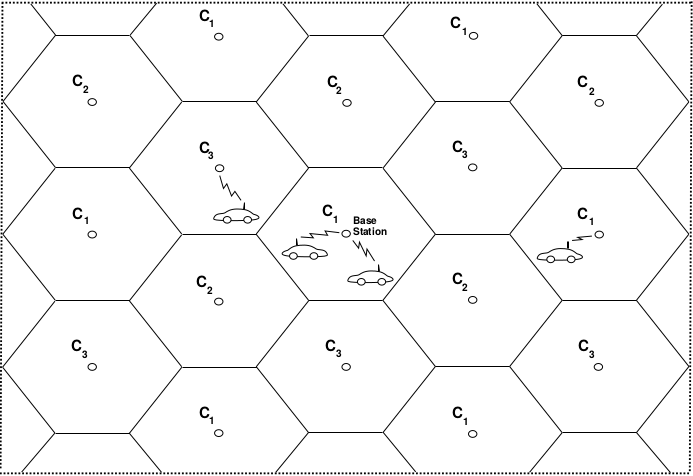
\includegraphics[width=0.8\textwidth]{figs/SistemaCelular.png}
	
	{Fonte: \cite{goldsmith2005wireless}.}
	\label{fig:Cells}
\end{figure}

\subsection{Algoritmos de alocação de recursos de rádio}

Uma das funções desempenhadas pelas BSs no enlace direto é a alocação dos recursos de rádio. Os algoritmos de RRA são responsáveis pela alocação dos recursos disponíveis de forma inteligente para que haja uma eficiente utilização desses recursos e que os requerimentos individuais de QoS de cada usuário sejam satisfeitos. Além disso, é desejável que os algoritmos de RRA maximizem a capacidade total do sistema \cite{gotsis2014radio}. Nesse contexto, alocar um recurso significa atribuir uma determinada faixa de frequência por um certo período de tempo a um determinado dispositivo móvel para que este receba uma transmissão de dados. Como cada recurso pode ser alocado para um determinado enlace entre uma BS e um dispositivo móvel, existe um grande número de possíveis alocações, mesmo que uma quantidade relativamente pequena de recursos e dispositivos móveis seja considerada \cite{maciel2010performance}.

Os algoritmos de RRA considerados neste trabalho funcionam da seguinte forma: no início de cada intervalo de tempo para transmissão de dados, a BS calcula a prioridade de cada usuário para um determinado recurso e então aquele recurso é alocado para o usuário com maior prioridade. Depois de alocar um determinado recurso, a BS continua a alocação até que todos os recursos tenham sido alocados ou que não exista mais usuários ativos para receber os recursos restantes \cite{Proc:Lei2007}.

Considerando a perspectiva das operadoras das redes celulares, atingir todos os objetivos citados acima significaria que a quantidade máxima possível de usuários estaria satisfeita e que houve um bom retorno dos investimentos, maximizando a receita. Olhando o ponto de vista dos usuários, é importante que ocorra uma justa alocação dos recursos e que eles possam satisfazer seus requerimentos de QoS, o que maximizaria sua satisfação \cite{Rodrigues2014_Wiley}.  

Em geral, esses algoritmos tentam se beneficiar das diversidades de frequência, múltiplos usuários, tempo e espaço proporcionadas pelas redes celulares baseadas em \acs{OFDMA}. Alguns algoritmos de RRA também utilizam algumas métricas dos usuários para determinar a prioridade dos mesmos na alocação dos recursos, tais como vazão de dados, atraso de pacotes, tamanho da fila de pacotes do usuário, entre outras métricas. Além disso, uma característica desejada que poderia estar presente em algoritmos de RRA é a flexibilidade para que as operadoras das redes celulares ajustem o ponto de operação dos algoritmos de acordo com decisões estratégicas ou segundo as mudanças de tendências dos clientes \cite{kim2009qos}. 

\subsection{Tipos de tráfego e satisfação do usuário}

Algumas aplicações RT presentes em redes celulares são sensíveis ao atraso, ou seja, são caracterizadas pela necessidade de um tempo de resposta curto entre as partes que estão se comunicando. Nesse tipo de aplicação, caso um determinado pacote de dados não chegue ao destinatário dentro de um determinado limite de tempo, este pacote é descartado, já que a informação contida naquele pacote não está mais temporalmente atualizada. Uma definição de satisfação do usuário comumente utilizada na literatura para este tipo de serviço é baseada na Taxa de Perda de Quadro (FER, do inglês \textit{Frame Erasure Rate}), que é uma razão entre a quantidade de pacotes descartados e o número total de pacotes gerados. Dessa maneira, um usuário é considerado satisfeito se sua \acs{FER} é igual ou menor que um determinado requerimento \cite{Rodrigues2014_Wiley}. Exemplos deste tipo de serviço são a aplicação de \acs{VoIP} e serviços de vídeo conferência.

Outra grande classe de serviços acessados por usuários de dispositivos móveis são os serviços NRT. Esta classe de serviços não possui requerimentos de atraso tão severos quanto os serviços RT, mas nesse tipo de aplicação não se tolera erro de pacotes. O pacote pode até demorar para chegar no destinatário, mas tem que chegar de maneira correta. Essas aplicações utilizam o Protocolo de Controle de Transporte (TCP, do inglês \textit{Transport Control Protocol}) na camada de transporte, o que garante esta confiabilidade \cite{Nasralla2013}. Usuários consumindo serviços NRT requerem que uma vazão de dados mínima seja mantida durante a sessão, portanto a satisfação desta classe de serviço é garantida se a vazão de dados da sessão for igual ou maior que um determinado requerimento. Exemplos desse tipo de serviço são as aplicações \acs{CBR}, navegação na Internet e e-mail.

Além das duas classes de serviços citadas acima, uma grande parcela do tráfego presente em redes celulares é oriundo de aplicações de vídeo. Para garantir que usuários utilizando serviços de vídeo tenham seus requerimentos de QoS atendidos, é necessário que a \acs{FER} dos usuários seja mantida abaixo de um determinado limite e que uma vazão de dados mínima seja mantida durante a sessão do vídeo \cite{basukala2009performance, Art:Andrews2001}. Portanto, um usuário deste tipo de serviço é considerado satisfeito se os dois requerimentos de QoS citados acima forem garantidos ao mesmo tempo.

\section{Objetivos}

\subsection{Objetivo geral}

O principal objetivo desta monografia é o estudo e avaliação do desempenho de algoritmos de alocação de recursos de rádio em cenários onde múltiplos serviços estão presentes. O estudo será conduzido por meio de simulações tendo como base os sistemas celulares da 4ª Geração baseados em {OFDMA}, onde existe imperfeição na estimação do estado do canal e existem usuários que estão utilizando serviços de classes diferentes. Dessa forma, o cenário analisado neste trabalho é complexo e possui características realistas encontradas nos ambientes cotidianos.

\subsection{Objetivos específicos}

Os objetivos específicos desta monografia são listados a seguir:

\begin{enumerate}
\item Estudo bibliográfico sobre algoritmos de alocação de recurso de rádio para sistemas celulares LTE de 4ª Geração, considerando cenários em que somente um serviço está presente ou cenários com múltiplos serviços;	 
\item Modelagem e implementação de um ambiente de simulação para sistemas celulares LTE de 4ª Geração baseados em {OFDMA}; 
\item Implementação da política de alocação de recursos de alguns algoritmos para análise de desempenho;
\item Análise de desempenho destes algoritmos por meio da métrica de satisfação do usuário para cenários onde somente um serviço está presente ou cenários com múltiplos serviços.
\end{enumerate}

\section{Organização da monografia}

Os estudos deste trabalho estão organizados da seguinte forma. No próximo capítulo será apresentado um extenso estudo bibliográfico sobre algoritmos de alocação de recursos de rádio para cenários com serviço único e múltiplos serviços. No capítulo \ref{Simulacao}, a modelagem do ambiente de simulação utilizado neste trabalho é descrita. No capítulo \ref{benchmarking} descrevemos os algoritmos que foram estudados mais a fundo e implementados para que seus desempenhos fossem analisados. No capítulo \ref{resultados} apresentamos o desempenho obtido pelos algoritmos estudados, classificando-os de acordo com a métrica de satisfação do usuário. Por fim, o último capítulo deste trabalho apresenta as conclusões tiradas a partir dos resultados obtidos e algumas perspectivas para a continuação deste trabalho. 